\documentclass[10pt, aspectratio=169]{beamer}

\usetheme{moloch}
\usecolortheme{default}

% Sfondo bianco
\setbeamercolor{background canvas}{bg=white}

% --- RIMOZIONE DELLE SLIDE DI SEZIONE ---
\AtBeginSection{} % Distrugge la creazione automatica del frame per le sezioni
\makeatletter
\setbeamertemplate{section page}{}
\def\beamer@aftersections{}{}
\makeatother

\usepackage[italian]{babel}
\usepackage{graphicx}
\usepackage{listings}
\usepackage{xcolor}
\usepackage{alltt}
\usepackage[most]{tcolorbox}
\tcbuselibrary{listings}
\usepackage{mathtools}
\usepackage{adjustbox}

% --- CONFIGURAZIONE COLORI CODICE ---
\definecolor{pyKeyword}{RGB}{0,90,180}
\definecolor{pyString}{RGB}{3,110,10}
\definecolor{pyComment}{RGB}{120,120,120}
\definecolor{pyOperator}{RGB}{180,0,90}

\definecolor{jvKeyword}{RGB}{166, 29, 41}
\definecolor{jvString}{RGB}{3, 47, 98}
\definecolor{jvComment}{RGB}{106, 115, 125}

\definecolor{goKeyword}{RGB}{0, 90, 180}
\definecolor{goString}{RGB}{3, 110, 10}
\definecolor{goComment}{RGB}{120, 120, 120}
\definecolor{goType}{RGB}{180, 0, 90}

\definecolor{flinkGenericColor}{RGB}{227, 26, 28}
\definecolor{flinkStreamColor}{RGB}{0, 102, 204}

% --- MACRO PER OBIETTIVI DELLE QUERY ---
\newcommand{\queryobjective}[1]{
    \vspace{-0.5cm}
    \begin{exampleblock}{\footnotesize Obiettivo}
    \scriptsize #1
    \end{exampleblock}
    \vfill
}

% --- CROP MACROS PER GRAFICI DI TELEMETRIA (GRAFANA SCREENSHOTS) ---
\newcommand{\CropThroughput}[1]{%
    \adjustbox{trim={0.01\width} {0.805\height} {0.00\width} {0.04\height}, clip}{%
        \includegraphics[width=\linewidth]{../Results/charts/#1}%
    }%
}
\newcommand{\CropLatency}[1]{%
    \adjustbox{trim={0.01\width} {0.455\height} {0.00\width} {0.308\height}, clip}{%
        \includegraphics[width=\linewidth]{../Results/charts/#1}%
    }%
}
\newcommand{\CropCheckpoint}[1]{%
    \adjustbox{trim={0.01\width} {0.348\height} {0.00\width} {0.55\height}, clip}{%
        \includegraphics[width=\linewidth]{../Results/charts/#1}%
    }%
}
\newcommand{\CropOutOfOrder}[1]{%
    \adjustbox{trim={0.01\width} {0.01\height} {0.00\width} {0.650\height}, clip}{%
        \includegraphics[width=\linewidth]{../Results/charts/#1}%
    }%
}
\newcommand{\CropNode}[1]{%
    \adjustbox{trim={0.01\width} {0.31\height} {0.00\width} {0.08\height}, clip}{%
        \includegraphics[width=\linewidth]{../Results/charts/#1}%
    }%
}

% --- IMPOSTAZIONI GLOBALI LISTINGS ---
\lstset{
    basicstyle=\ttfamily\fontsize{5pt}{6.5pt}\selectfont,
    backgroundcolor=,
    frame=none,
    breaklines=true,
    breakatwhitespace=true,
    showstringspaces=false,
    xleftmargin=2pt,
    xrightmargin=2pt
}

% --- STILE PYTHON ---
\lstdefinestyle{Python}{
    language=Python,
    keywordstyle=\color{pyKeyword}\bfseries,
    stringstyle=\color{pyString},
    commentstyle=\color{pyComment}\itshape,
    morekeywords=[2]{TelegrafConsumer},
    keywordstyle=[2]\color{pyOperator}\bfseries
}

% --- STILE GO ---
\lstdefinestyle{Go}{
    language=Go,
    keywordstyle=\color{goKeyword}\bfseries,
    stringstyle=\color{goString},
    commentstyle=\color{goComment}\itshape,
    morekeywords={go, chan, select, defer, type, struct, interface, package, import, func, return, var, const},
    keywordstyle=[2]\color{goType}\bfseries,
    morekeywords=[2]{string, int, int64, float64, bool, error}
}

% --- STILE JAVA BASE ---
\lstdefinestyle{JavaBase}{
    language=Java,
    keywordstyle=\color{jvKeyword}\bfseries,
    stringstyle=\color{jvString},
    commentstyle=\color{jvComment}\itshape,
    morekeywords=[4]{Tuple2, Tuple3, Row, List, Map, Collector, Context, RuntimeContext, Configuration, PerformanceMetrics, SimpleStringSchema},
    keywordstyle=[4]\color{blue!80!black}\bfseries
}

% --- STILE JAVA FLINK ---
\lstdefinestyle{JavaFlink}{
    style=JavaBase,
    morekeywords=[2]{map, filter, keyBy, window, trigger, aggregate, process, addSource, addSink, getRuntimeContext, getState},
    keywordstyle=[2]\color{flinkStreamColor}\bfseries,
    morekeywords=[3]{DataStream, KeyedStream, WindowedStream, SingleOutputStreamOperator, StreamExecutionEnvironment, KafkaSource, KafkaSink, AggregateFunction, ProcessWindowFunction, KeyedProcessFunction, MapState, ValueState, DDSketch, BoundedOutOfOrdernessWatermarks, WatermarkStrategy},
    keywordstyle=[3]\color{flinkGenericColor}\bfseries
}

% --- STILE PER TERMINALE ---
\lstdefinestyle{Terminal}{
    language=bash,
    basicstyle=\ttfamily\scriptsize\color{white}, 
    keywordstyle=\color{white},                   
    stringstyle=\color{white},
    commentstyle=\color{gray},
    breaklines=true,
    extendedchars=true,
    literate={textdollar}{{\$}}1               
}

% --- CONFIGURAZIONE BASE BOX ---
\tcbset{
    codeboxbase/.style={
        listing only,
        arc=5pt,
        boxrule=0.8pt,
        fonttitle=\scriptsize\bfseries\sffamily,
        top=8pt, bottom=1pt, left=1pt, right=1pt,
        toptitle=3pt, bottomtitle=3pt, lefttitle=6pt, righttitle=6pt,
        enhanced,
        attach boxed title to top left={yshift=-2mm, xshift=2mm},
        boxed title style={sharp corners, boxrule=0.5pt}
    }
}

% --- BOX CODICE PERSONALIZZATI ---

% Box per codice Go - Tema Teal
\newtcblisting{gocodebox}[1]{
    codeboxbase,
    listing options={style=Go, aboveskip=0pt, belowskip=0pt, extendedchars=true},
    colframe=teal!30!black!30,
    colback=teal!2,
    title={#1},
    coltitle=teal!80!black,
    colbacktitle=teal!12,
    boxed title style={sharp corners, boxrule=0.5pt, colframe=teal!30!black!30}
}

% Box per codice Flink - Tema Magenta/Flink
\newtcblisting{flinkcodebox}[1]{
    codeboxbase,
    listing options={style=JavaFlink, aboveskip=0pt, belowskip=0pt},
    colframe=magenta!30!black!30,
    colback=magenta!2,
    title={#1},
    coltitle=magenta!80!black,
    colbacktitle=magenta!12,
    boxed title style={sharp corners, boxrule=0.5pt, colframe=magenta!30!black!30}
}

% Box per codice Java generico - Tema Grigio/Azzurro
\newtcblisting{appcodebox}[1]{
    codeboxbase,
    listing options={style=JavaBase, aboveskip=0pt, belowskip=0pt},
    colframe=blue!20!gray!60,
    colback=blue!2!white,
    title={#1},
    coltitle=blue!40!black,
    colbacktitle=blue!10!gray!10,
    boxed title style={sharp corners, boxrule=0.5pt, colframe=blue!20!gray!60}
}

% Box per codice Python
\newtcblisting{pythoncodebox}[1]{
    codeboxbase,
    listing options={style=Python, aboveskip=0pt, belowskip=0pt, extendedchars=true},
    colframe=black!25,
    colback=black!2,
    title={#1},
    coltitle=black!85,
    colbacktitle=black!8,
    boxed title style={sharp corners, boxrule=0.5pt, colframe=black!25}
}

% Box per terminale
\newtcblisting{terminalbox}[1]{
    listing only,
    listing options={style=Terminal, aboveskip=0pt, belowskip=0pt},
    arc=5pt,
    boxrule=0.5pt,
    colframe=black!80,
    colback=black!85,           
    title={#1},
    coltitle=white,        
    colbacktitle=black!70,                   
    fonttitle=\scriptsize\bfseries\sffamily,
    top=2pt, bottom=2pt, left=2pt, right=2pt, 
    toptitle=4pt, bottomtitle=4pt
}

% --- METADATI TITOLO ---
\title[Sky Analytics Stream]{Sky Analytics Stream}
\subtitle{Architettura Distribuita per l'Analisi in Tempo Reale del Traffico Aereo}
\author[Simonelli, Masci]{Flavio Simonelli \and Francesco Masci}
\institute[SABD]{
    Corso Architettura e Sistemi per Big Data\\
    Corso di Laurea Magistrale in Ingegneria Informatica\\
    Università di Roma "Tor Vergata"
}
\date[Luglio 2026]{Luglio 2026}

\titlegraphic{
\includegraphics[width=2cm]{logos/logo_tor_vergata}}

\begin{document}

% Macro per slide di transizione di sezione
\newcommand{\SectionFrame}[2][]{%
    \begin{frame}[plain]
        \vfill
        \begin{center}
            {\Huge\bfseries #2\par}
            \vspace{0.45cm}
            {\small\color{black!60}\begin{minipage}{0.78\textwidth}\centering #1\end{minipage}\par}
        \end{center}
        \vfill
    \end{frame}
}

% Slide iniziale di avviso
\begin{frame}[plain]
    \vfill
    \begin{center}
        {\Huge\bfseries Le slide sono in fase di elaborazione\par}
        \vspace{0.8cm}
        {\LARGE verranno consegnate dopo la presentazione come richiesto\par}
    \end{center}
    \vfill
\end{frame}

% Slide del Titolo
\begin{frame}
    \titlepage
\end{frame}

% Slide dell'Indice
\begin{frame}{Indice}
    \vspace{-0.3cm}
    \begin{columns}[T]
        \begin{column}{0.48\textwidth}
            \begin{enumerate}
                \item \textbf{Architettura e Flusso}
                \\{\scriptsize Stack tecnologico ed interazione delle componenti}
                \vspace{0.35cm}

                \item \textbf{Ingestion e Broker Layer}
                \\{\scriptsize Simulatore Go, buffer di Kafka e partizionamento}
                \vspace{0.35cm}

                \item \textbf{Stream Processing Core}
                \\{\scriptsize Apache Flink: watermarks, POJO, percentili e query}
            \end{enumerate}
        \end{column}

        \begin{column}{0.48\textwidth}
            \begin{enumerate}\setcounter{enumi}{3}
                \item \textbf{Infrastruttura di Deployment}
                \\{\scriptsize Container locali ed AWS CloudFormation con Route 53}
                \vspace{0.35cm}

                \item \textbf{Valutazione Sperimentale}
                \\{\scriptsize Parallelismo, disordine temporale e checkpointing}
                \vspace{0.35cm}

                \item \textbf{Risultati Analitici}
                \\{\scriptsize Analisi dei ritardi, granularità ed effetto della perdita dati}
            \end{enumerate}
        \end{column}
    \end{columns}
\end{frame}

% --- SEZIONE 1 ---
\section{Architettura e Flusso}\label{sec:architecture_and_flow}
\SectionFrame[Panoramica del sistema streaming ed interazione asincrona tra il generatore di carico, il message broker, Flink e lo stack di persistenza e visualizzazione.]{Architettura e Flusso}

\begin{frame}{Big Data Stack e Flow Diagram}
    \begin{columns}[c]
        \begin{column}{0.48\textwidth}
            \centering
            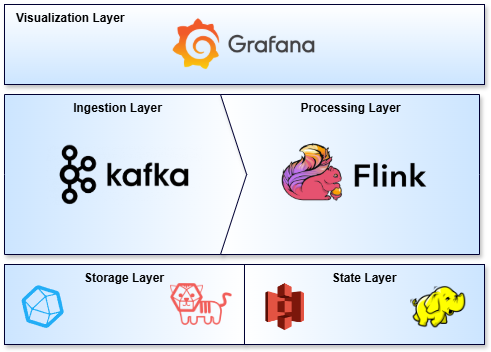
\includegraphics[width=\linewidth,height=0.68\textheight,keepaspectratio]{../Report/graphs/BigDataStack.png}
            \vskip 0.2cm
            \small Componenti del Big Data Stack
        \end{column}

        \begin{column}{0.48\textwidth}
            \centering
            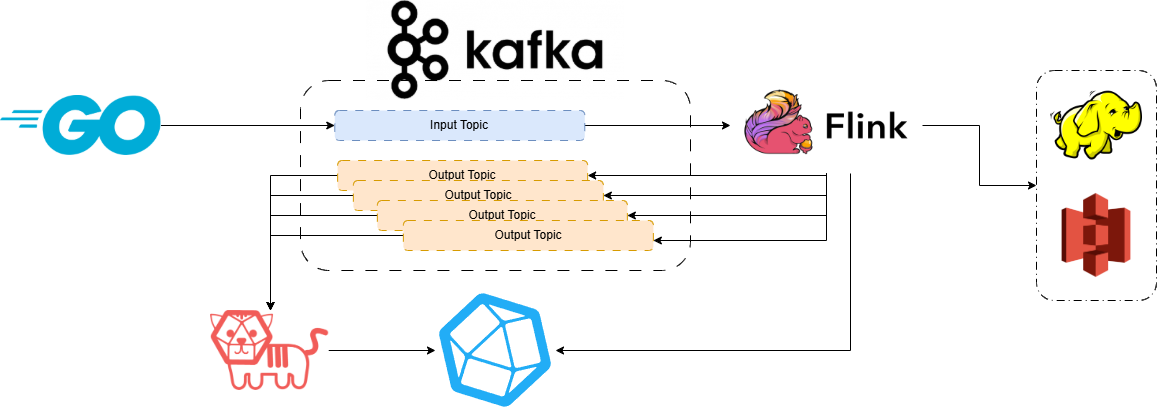
\includegraphics[width=\linewidth,height=0.68\textheight,keepaspectratio]{../Report/graphs/InteractionDiagram.png}
            \vskip 0.2cm
            \small Diagramma di interazione e flussi dati
        \end{column}
    \end{columns}
\end{frame}

% --- SEZIONE 2 ---
\section{Ingestion e Broker Layer}\label{sec:ingestion_and_broker_layer}
\SectionFrame[Il simulatore custom in Go per la generazione di flussi accelerati e disordinati ed il buffering distribuito basato su partizionamento Kafka.]{Ingestion e Broker Layer}

\begin{frame}[fragile]{Ingestione: Il Simulatore Custom in Go}
    \begin{columns}[c]
        \begin{column}{0.54\textwidth}
            \begin{itemize}
                \item \textbf{Razionale delle performance}: Scritto in Go per azzerare l'impatto del Garbage Collector e massimizzare il throughput.
                \item \textbf{Ottimizzazioni startup}: Decompressione automatica e ordinamento in event-time archiviati in cache binaria \texttt{.gob}.
                \item \textbf{Temporizzazione Ibrida}: CPU rilasciata per lunghe attese, attesa attiva (*busy wait*) per precisione a livello di millisecondo sui flussi accelerati.
                \item \textbf{Disordine Controllato}: Iniezione casuale controllata di ritardi per testare la tolleranza ai dati fuori ordine.
            \end{itemize}
        \end{column}

        \begin{column}{0.44\textwidth}
            \begin{block}{\scriptsize Scenari di Accelerazione}
                \centering
                \fontsize{5.5pt}{7pt}\selectfont
                \begin{tabular}{lccc}
                    \hline
                    \textbf{Parametro} & \textbf{Lento} & \textbf{Medio} & \textbf{Alto} \\
                    \hline
                    \textbf{Target} & 1.440x & 14.400x & 43.200x \\
                    \textbf{Rapporto} & 1g/1m & 10g/1m & 30g/1m \\
                    \textbf{Durata} & $\approx$ 120m & $\approx$ 12m & $\approx$ 4m \\
                    \textbf{Nominale} & $\approx$ 305 ev/s & $\approx$ 3.050 ev/s & $\approx$ 9.150 ev/s \\
                    \textbf{Reale} & $\approx$ 302 ev/s & $\approx$ 2.928 ev/s & $\approx$ 8.200 ev/s \\
                    \hline
                \end{tabular}
            \end{block}
            \vfill
            \begin{gocodebox}{Go - Iniezione Disordine (Pseudo)}
if rand.Float64() < p.oooProb {
    offset := rand.Int64n(p.maxDelayMin)
    eventTime = eventTime.Add(-offset)
}
// Ordinamento per tempo reale di invio
            \end{gocodebox}
        \end{column}
    \end{columns}
\end{frame}

\begin{frame}[fragile]{Message Broker: Apache Kafka}
    \begin{columns}[c]
        \begin{column}{0.50\textwidth}
            \textbf{Partizionamento e Parallelismo}
            \begin{itemize}
                \item Topic primario \texttt{flights-stream} configurato con 6 partizioni.
                \item Permette uno scale-out lineare di Flink (mapping 1:1 ottimale tra partizioni e consumer subtask).
            \end{itemize}

            \textbf{Scrittura bilanciata in Ingress}
            \begin{itemize}
                \item Scrittura in \textit{Round-Robin} (chiave nulla) dal simulatore.
                \item Distribuzione uniforme del carico: previene la formazione di *idle partitions* (che arresterebbero l'avanzamento dei watermark in Flink) o *hot partitions*.
            \end{itemize}

            \textbf{Instradamento dell'Output}
            \begin{itemize}
                \item Topic dedicati per query e finestre.
                \item Scrittura partizionata per chiave (`airline` o `origin\_airport\_id`) per consentire letture cronologiche parziali a valle.
            \end{itemize}
        \end{column}

        \begin{column}{0.48\textwidth}
            \begin{terminalbox}{Terminale - Creazione Topic Kafka}
kafka-topics.sh --create --bootstrap-server kafka:9092 \
    --partitions 6 --replication-factor 3 \
    --topic flights-stream

kafka-topics.sh --create --bootstrap-server kafka:9092 \
    --partitions 3 --replication-factor 3 \
    --topic flights-q1-results
            \end{terminalbox}
        \end{column}
    \end{columns}
\end{frame}

% --- SEZIONE 3 ---
\section{Stream Processing Core (Apache Flink)}\label{sec:stream_processing_core}
\SectionFrame[Architettura della topologia computazionale concorrente, gestione del tempo logico, ottimizzazioni di memoria, DDSketch e dettagli delle query.]{Stream Processing con Apache Flink}

\begin{frame}[fragile]{Configurazione Job e Ottimizzazione POJO}
    \begin{columns}[c]
        \begin{column}{0.54\textwidth}
            \textbf{Topologia a Sorgente Condivisa}
            \begin{itemize}
                \item Unica istanza di `KafkaSource` condivisa tra le tre query.
                \item I filtri di data quality (scarto record nulli, logicamente incoerenti) vengono eseguiti una sola volta a monte, azzerando l'I/O e la deserializzazione ridondante.
            \end{itemize}

            \textbf{Modellazione a POJO e PojoSerializer}
            \begin{itemize}
                \item Classe `FlightRecord` implementata rigorosamente come POJO (costruttore vuoto pubblico, attributi non-final, getter/setter).
                \item Flink evita la costosa serializzazione basata su Kryo.
                \item Generazione automatica di `PojoSerializer`: posizionamento fisso dei byte che riduce lo stato in RocksDB e velocizza lo shuffle di rete.
            \end{itemize}
        \end{column}

        \begin{column}{0.44\textwidth}
            \begin{flinkcodebox}{Flink Job Configuration (Java)}
StreamExecutionEnvironment env = 
    StreamExecutionEnvironment.getExecutionEnvironment();

env.getConfig().enableForceAvro(); // Disabilita Kryo
env.getConfig().enableGenericTypes();

DataStream<FlightRecord> stream = env
    .fromSource(kafkaSource, WatermarkStrategy.noWatermarks(), ...)
    .filter(new DataQualityFilter());
            \end{flinkcodebox}
        \end{column}
    \end{columns}
\end{frame}

\begin{frame}[fragile]{Gestione del Disordine e Qualità del Dato}
    \begin{columns}[c]
        \begin{column}{0.52\textwidth}
            \textbf{Normalizzazione del dato}
            \begin{itemize}
                \item I record con ritardi mancanti vengono impostati a zero (assunzione conservativa di puntualità).
            \end{itemize}
            \textbf{Sincronizzazione in Event-Time}
            \begin{itemize}
                \item \textbf{Bounded-Out-of-Orderness}: Ritardo massimo del watermark configurabile a start-time via YAML.
                \item \textbf{Idleness Detection}: Le partizioni Kafka inattive vengono marcate come temporaneamente *idle* per non bloccare il watermark globale.
                \item \textbf{Allowed Lateness}: Le finestre accumulano record tardivi entro una tolleranza extra, emettendo aggiornamenti incrementali.
                \item \textbf{Side Outputs}: I record definitivamente tardivi vengono deviati in canali di telemetria dedicati.
            \end{itemize}
        \end{column}

        \begin{column}{0.46\textwidth}
            \begin{flinkcodebox}{Flink Watermarking \& Lateness}
WatermarkStrategy<FlightRecord> strategy =
    WatermarkStrategy.<FlightRecord>forBoundedOutOfOrderness(
        Duration.ofMinutes(config.getWatermarkDelayMin())
    )
    .withTimestampAssigner((event, timestamp) -> event.getEventTime())
    .withIdleness(Duration.ofSeconds(10));

DataStream<FlightRecord> timedStream = 
    stream.assignTimestampsAndWatermarks(strategy);

windowedStream
    .allowedLateness(Time.minutes(config.getAllowedLatenessMin()))
    .sideOutputLateData(lateTag)
            \end{flinkcodebox}
        \end{column}
    \end{columns}
\end{frame}

\begin{frame}[fragile]{Fault Tolerance e Garanzie di Consegna E2E}
    \begin{columns}[c]
        \begin{column}{0.54\textwidth}
            \textbf{Exactly-Once Interno}
            \begin{itemize}
                \item Snapshot asincroni barriera-basati (algoritmo di Chandy-Lamport).
                \item Salvataggio persistente su storage distribuito (HDFS locale / Amazon S3 su cloud).
                \item In caso di crash, lo stato degli operatori e degli accumulatori delle finestre viene ripristinato esattamente alla barriera pre-fallimento.
            \end{itemize}
            \textbf{Garanzie End-to-End Ibride}
            \begin{itemize}
                \item Il Sink Kafka è impostato a \textit{At-Least-Once} (per evitare il forte overhead del protocollo transazionale distributed 2PC).
                \item A valle, InfluxDB agisce in modalità idempotente: i duplicati generati dal restore di Flink presentano chiavi primarie e timestamp identici, sovrascrivendo i record precedenti.
                \item \textbf{Risultato}: Garanzia matematica dell'Exactly-Once End-to-End con throughput nativo.
            \end{itemize}
        \end{column}

        \begin{column}{0.44\textwidth}
            \centering
            \begin{block}{\scriptsize Configurazione Checkpoint}
                \begin{flinkcodebox}{Java Checkpointing Configuration}
env.enableCheckpointing(30000); // 30s
env.getCheckpointConfig()
  .setCheckpointingMode(CheckpointingMode.EXACTLY_ONCE);
env.getCheckpointConfig()
  .setMinPauseBetweenCheckpoints(10000); // 10s
env.getCheckpointConfig()
  .setExternalizedCheckpointCleanup(
    ExternalizedCheckpointCleanup.RETAIN_ON_CANCELLATION
  );
                \end{flinkcodebox}
            \end{block}
        \end{column}
    \end{columns}
\end{frame}

\begin{frame}[fragile, t]{Query 1: Analisi Performance Compagnie}
    \queryobjective{Calcolare per ciascuna compagnia aerea, su finestre temporali di 1 ora, la media oraria dei ritardi in partenza ed il tasso di cancellazione dei voli.}
    
    \begin{flinkcodebox}{Query 1 implementation: AggregateFunction}
DataStream<Query1Result> q1 = stream
    .keyBy(FlightRecord::getAirline)
    .window(TumblingEventTimeWindows.of(Time.hours(1)))
    .aggregate(new Q1Aggregator(), new Q1WindowProcessor());

// Q1Aggregator implements AggregateFunction<FlightRecord, Q1Accumulator, Q1Output>
// Q1Accumulator mantiene: totalFlights, cancelledFlights, sumDelay.
// Complessita spaziale e computazionale: O(1) ad inserimento, aggregazione incrementale nello stato
    \end{flinkcodebox}
    \vfill
    \begin{columns}[T]
        \begin{column}{0.48\textwidth}
            \begin{block}{\scriptsize Accumulatore locale (O(1))}
                Ad ogni record: \texttt{acc.total++}. Se cancellato: \texttt{acc.cancelled++}. Altrimenti: \texttt{acc.sumDelay += r.getDepDelay()}.
            \end{block}
        \end{column}
        \begin{column}{0.48\textwidth}
            \begin{block}{\scriptsize Processamento di finestra}
                Calcola al trigger: \texttt{avgDelay = sumDelay / (total - cancelled)} e \texttt{cancelRate = (cancelled / total) * 100}.
            \end{block}
        \end{column}
    \end{columns}
\end{frame}

\begin{frame}[fragile, t]{Query 2: Top-10 Aeroporti con Ritardi Severi}
    \queryobjective{Classifica in tempo reale dei 10 aeroporti con il maggior numero di ritardi gravi (delay > 15 minuti) su tre finestre temporali parallele: 1 ora tumbling, 6 ore tumbling e finestra globale ad aggiornamento orario.}
    
    \begin{flinkcodebox}{Query 2: Pattern Local-Global Aggregation \& Min-Heap}
// Fase 1: Aggregazione Locale per Aeroporto
DataStream<AirportDelayCount> localCounts = stream
    .filter(r -> r.getArrDelay() > 15)
    .keyBy(FlightRecord::getOriginAirport)
    .window(TumblingEventTimeWindows.of(Time.hours(1)))
    .sum("delayCount"); // Calcolo incrementale locale

// Fase 2: Classifica Globale con KeyedProcessFunction
DataStream<Top10Airports> globalTop10 = localCounts
    .keyBy(AirportDelayCount::getWindowEnd)
    .process(new Top10ProcessFunction()); 

// Top10ProcessFunction colleziona i conteggi in MapState. All'attivazione del timer su watermark:
// 1. Estrae i record ed inserisce in un Min-Heap prioritario limitato a 10 elementi: O(N log 10)
// 2. Emette la classifica ordinata decrescente e svuota MapState per liberare la memoria dello stato
    \end{flinkcodebox}
\end{frame}

\begin{frame}[fragile, t]{Query 3: Percentili dei Ritardi e DDSketch}
    \queryobjective{Calcolo dei percentili (25-esimo, 50-esimo, 75-esimo, 90-esimo) dei ritardi in partenza per compagnia e fascia oraria su tre finestre temporali: 24 ore tumbling, 7 giorni tumbling e globale ad aggiornamento giornaliero.}
    
    \begin{flinkcodebox}{Query 3: DDSketch Integration in State}
DataStream<Query3Result> q3 = stream
    .keyBy(r -> Tuple2.of(r.getAirline(), r.getHourOfDay()))
    .window(TumblingEventTimeWindows.of(Time.days(1)))
    .process(new Q3DDSketchProcessFunction());

// Q3DDSketchProcessFunction mappa i ritardi in bin logaritmici: i = ceil( log_gamma(x) )
// gamma = (1 + alpha) / (1 - alpha), con alpha = 0.01 (errore relativo garantito 1%)
// Stima quantile q nel bin i: x_q = ( 2 * gamma^i ) / (gamma + 1)
// DDSketch memorizza solo le frequenze dei bin (dimensione massima m = 2048 bin): footprint memoria costante e O(1) mergeability
    \end{flinkcodebox}
    \vfill
    \begin{columns}[T, onlytextwidth]
        \begin{column}{0.48\textwidth}
            \begin{block}{\scriptsize Vantaggio Computazionale}
                Accuratezza eccellente sulle code di distribuzioni asimmetriche con costi spaziali limitati rispetto a KLL o UDDSketch.
            \end{block}
        \end{column}
        \begin{column}{0.48\textwidth}
            \begin{block}{\scriptsize Tolleranza all'Errore}
                Un errore dell'1\% equivale a $\approx 36$ secondi su 1 ora di ritardo: trascurabile per l'analisi del traffico aereo.
            \end{block}
        \end{column}
    \end{columns}
\end{frame}

\begin{frame}[fragile]{Sistema di Osservabilità e Telemetria}
    \begin{columns}[c]
        \begin{column}{0.54\textwidth}
            \textbf{Raccolta delle Metric API di Flink}
            \begin{itemize}
                \item \textbf{Data Quality}: Counter cumulativo dei record scartati per anomalie di business.
                \item \textbf{Record Tardivi}: Counter per i record scartati oltre l'allowed lateness, gauge per la lateness massima e percentili di lateness stimati con DDSketch.
                \item \textbf{Latenza end-to-end}: Calcolo al trigger di finestra tramite i timestamp di ingestion nel sistema:
                \begin{itemize}
                    \item \textit{Newest E2E Latency}: Tempo di transito del record più recente.
                    \item \textit{Oldest E2E Latency}: Tempo di transito del record più vecchio.
                    \item \textit{Average E2E Latency}: Latenza media dei record della finestra.
                \end{itemize}
            \end{itemize}
            \textbf{Bypass del Broker per le Metriche}
            \begin{itemize}
                \item Integrazione nativa di `InfluxdbReporterFactory`.
                \item Flink invia le telemetrie in modalità asincrona a InfluxDB direttamente, risparmiando banda a Kafka.
            \end{itemize}
        \end{column}

        \begin{column}{0.44\textwidth}
            \begin{block}{\scriptsize Metric Registration in Flink (Java)}
                \begin{alltt}
public class TelemetryMapper extends RichMapFunction<...> {
    private transient Counter discardedCounter;
    private transient Gauge<Long> e2eLatencyGauge;

    @Override
    public void open(Configuration parameters) {
        this.discardedCounter = getRuntimeContext()
            .getMetricGroup()
            .counter("discarded_records_count");
    }
}
                \end{alltt}
            \end{block}
        \end{column}
    \end{columns}
\end{frame}

% --- SEZIONE 4 ---
\section{Infrastruttura di Deployment}\label{sec:deployment_infrastructure}
\SectionFrame[Architettura multi-container locale ed automazione cloud del cluster distribuito su AWS EC2 tramite CloudFormation e Route 53.]{Infrastruttura di Deployment}

\begin{frame}{Deployment Locale vs AWS Cloud}
    \begin{columns}[T]
        \begin{column}{0.48\textwidth}
            \centering
            \textbf{Locale (Docker Compose)}
            \begin{itemize}
                \item Rete private bridge per l'interconnessione di 11 container.
                \item 1 broker Kafka + container init.
                \item Flink JobManager + 3 TaskManager (2 slot ciascuno $\rightarrow$ parallelismo max 6).
                \item 3 container HDFS (1 NameNode, 2 DataNode) per checkpointing simulato.
                \item Telegraf + InfluxDB + Grafana per persistenza e visualizzazione.
                \item Configurazione iniettata via file \texttt{.env}.
            \end{itemize}
        \end{column}

        \begin{column}{0.48\textwidth}
            \centering
            \textbf{AWS Distributed Cloud}
            \begin{itemize}
                \item Provisioning automatizzato tramite stack AWS CloudFormation.
                \item VPC dedicata con Private Hosted Zone su Amazon Route 53 (\texttt{flight-analysis.local}) per risoluzione DNS interna senza IP fissi.
                \item Bootstrap automatico delle istanze EC2 all'avvio: installazione Docker, download delle build da S3 e deploy.
            \end{itemize}
            \vfill
            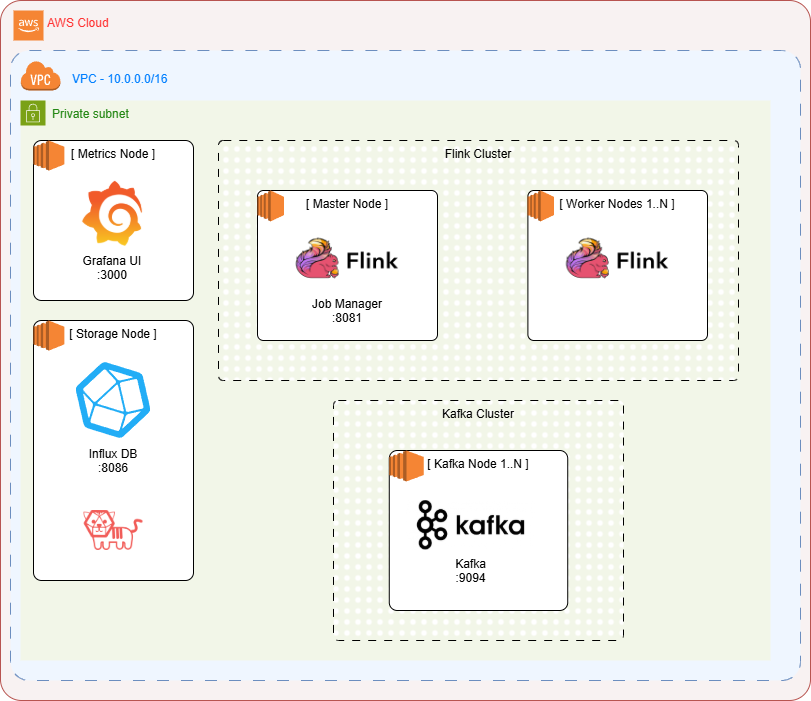
\includegraphics[width=\linewidth,height=0.45\textheight,keepaspectratio]{../Report/graphs/DeploymentView-EC2.png}
        \end{column}
    \end{columns}
\end{frame}

\begin{frame}{Dimensionamento delle Istanze EC2}
    \begin{columns}[c]
        \begin{column}{0.54\textwidth}
            \textbf{Scelta delle Famiglie EC2}
            \begin{itemize}
                \item Per i nodi computazionali di Flink sono state evitate istanze burstable (famiglia \texttt{t3}) per eliminare il rischio di CPU throttling sotto carico da esaurimento crediti.
                \item Scelta ricaduta sulle istanze compute-optimized della famiglia \textbf{\texttt{c6i}}.
            \end{itemize}
            \textbf{Topologia del Cluster AWS}
            \begin{itemize}
                \item \textbf{Flink JobManager}: 1 x \texttt{c6i.large} (2 vCPU, 4 GiB RAM).
                \item \textbf{Flink TaskManager}: 3 x \texttt{c6i.large} (2 vCPU, 4 GiB RAM, 2 slot ciascuno).
                \item \textbf{Kafka Cluster}: 1 x \texttt{t3.large} (broker master e generatore simulatore) + 2 x \texttt{t3.medium} (repliche).
                \item \textbf{Persistenza e Grafica}: 2 x \texttt{t3.small} (Telegraf/InfluxDB, Grafana).
            \end{itemize}
        \end{column}

        \begin{column}{0.44\textwidth}
            \begin{block}{\scriptsize Risoluzione DNS Interna}
                \centering
                \scriptsize
                \begin{tabular}{ll}
                    \hline
                    \textbf{Hostname DNS} & \textbf{Ruolo} \\
                    \hline
                    \texttt{kafka1.flight-analysis.local} & Kafka Master \\
                    \texttt{kafka2.flight-analysis.local} & Kafka Repl 1 \\
                    \texttt{jobmanager.flight-analysis.local} & Flink JM \\
                    \texttt{taskmanager1.flight-analysis.local} & Flink TM 1 \\
                    \texttt{influxdb.flight-analysis.local} & InfluxDB \\
                    \hline
                \end{tabular}
            \end{block}
        \end{column}
    \end{columns}
\end{frame}

% --- SEZIONE 5 ---
\section{Valutazione Sperimentale}\label{sec:experimental_evaluation}
\SectionFrame[Campagne sperimentali condotte sul cluster cloud AWS: analisi di parallelismo e scalabilità, impatto del disordine temporale ed overhead del checkpointing.]{Valutazione Sperimentale}

\begin{frame}{Parallelismo e Scalabilità: Analisi del Throughput}
    \begin{columns}[T]
        \begin{column}{0.48\textwidth}
            \centering
            \textbf{Scenario Fast: Transitorio}
            \vskip 0.1cm
            \CropThroughput{cluster_clean_run_fast_para3_part6.png}
            \vskip 0.1cm
            {\tiny Throughput scenario Fast con parallelismo P=3}
        \end{column}

        \begin{column}{0.48\textwidth}
            \textbf{Discussione dei Risultati}
            \begin{itemize}
                \footnotesize
                \item \textbf{Scenari Slow \& Medium}: Il throughput in ingresso è limitato dalla sorgente ($\approx 300$ ev/s e $\approx 3.000$ ev/s). $P=1$ è già sovradimensionato: lo scale-out non porta incrementi.
                \item \textbf{Scenario Fast}: L'ingestion si stabilizza a regime a $\approx 8.500$ ev/s indipendentemente da $P$.
                \item Tuttavia, il throughput in uscita a regime aumenta all'aumentare di $P$:
                \begin{itemize}
                    \scriptsize
                    \item $P=1$: $\approx 236$ record/s.
                    \item $P=6$: $\approx 280\text{--}288$ record/s.
                \end{itemize}
                \item \textbf{Razionale}: In uno stream accelerato, finestre logiche molto dense vengono compresse in pochi millisecondi reali; la presenza di slot paralleli ottimizza lo svuotamento simultaneo delle finestre abbattendo i picchi di emissione.
            \end{itemize}
        \end{column}
    \end{columns}
\end{frame}

\begin{frame}{Parallelismo e Scalabilità: Analisi delle Latenze}
    \begin{columns}[T]
        \begin{column}{0.48\textwidth}
            \centering
            \textbf{Watermark Drift ad Alto Parallelismo ($P=6$)}
            \vskip 0.1cm
            \CropLatency{cluster_clean_run_medium_para6_part6.png}
            \vskip 0.1cm
            {\tiny Latenza E2E P90 scenario Medium con parallelismo P=6}
        \end{column}

        \begin{column}{0.48\textwidth}
            \textbf{Analisi del Watermark Drift}
            \begin{itemize}
                \footnotesize
                \item \textbf{Parallelismo $P=1$ e $P=3$}: Curve piatte e stabili durante l'intera run. La latenza P90 si attesta a $\approx 2.25$ secondi reali nello scenario Fast.
                \item \textbf{Parallelismo $P=6$}: Presenza di picchi impulsivi transitori sia nello scenario Medium (fino a $18.5$ secondi per la Q3 7d e $12.5$s per la Q3 Global) sia in quello Fast ($6.5$ secondi).
                \item \textbf{Causa logica}: La frammentazione dello stream su 6 slot paralleli accentua il disallineamento temporaneo dei watermark tra i subtask (*watermark drift*). Il coordinamento richiede la sincronizzazione sul watermark più lento; questo introduce ritardi transitori che si risolvono autonomamente non appena i watermark convergono, escludendo fenomeni di lag cumulativo permanente.
            \end{itemize}
        \end{column}
    \end{columns}
\end{frame}

\begin{frame}{Gestione del Disordine Temporale}
    \begin{columns}[T]
        \begin{column}{0.48\textwidth}
            \centering
            \textbf{Out-of-orderness e Latenza}
            \vskip 0.1cm
            \CropOutOfOrder{cluster_delay_run_d30_l0.png}
            \vskip 0.1cm
            {\tiny Statistiche di out-of-orderness con D=30 min e L=0}
        \end{column}

        \begin{column}{0.48\textwidth}
            \textbf{Trade-off: Completezza vs Latenza}
            \begin{itemize}
                \footnotesize
                \item \textbf{Aggressivo ($D=10$ min, $L=0$ min)}:
                \begin{itemize}
                    \scriptsize
                    \item Finestre chiuse rapidamente (bassa latenza).
                    \item Elevata percentuale di record scartati perché giunti oltre la tolleranza.
                \end{itemize}
                \item \textbf{Ibrido ($D=5$ min, $L=25$ min)}:
                \begin{itemize}
                    \scriptsize
                    \item Chiusura rapida delle finestre ma stato mantenuto in memoria per ulteriori 25 minuti.
                    \item Emette aggiornamenti tardivi incrementali salvando la completezza analitica.
                \end{itemize}
                \item \textbf{Conservativo ($D=30$ min, $L=0$ min)}:
                \begin{itemize}
                    \scriptsize
                    \item Garanzia di massima completezza senza scarti.
                    \item Pagamento di una penalità fissa sulla latenza di emissione: le finestre rimangono aperte 30 minuti logici in più.
                \end{itemize}
            \end{itemize}
        \end{column}
    \end{columns}
\end{frame}

\begin{frame}{Impatto del Checkpointing e Resilienza}
    \begin{columns}[T]
        \begin{column}{0.48\textwidth}
            \centering
            \textbf{Test di Failover e Ripristino dello Stato}
            \vskip 0.1cm
            \CropThroughput{cluster_chk_hashmap_run_int5_fail1.png}
            \vskip 0.1cm
            {\tiny Throughput durante failover (checkpoint 5 min, 1 crash)}
        \end{column}

        \begin{column}{0.48\textwidth}
            \textbf{Overhead e Dinamiche di Recovery}
            \begin{itemize}
                \footnotesize
                \item \textbf{Overhead di Scrittura}: Il checkpointing frequente (30s vs 5m) introduce una riduzione impercettibile del throughput stazionario e mantiene stabili le latenze P90.
                \item \textbf{Dinamica di Crash/Restore}:
                \begin{itemize}
                    \scriptsize
                    \item \textbf{Crash}: Al minuto 6:30 viene terminato forzatamente un TaskManager. Il throughput crolla a zero e Kafka accumula lag in ingresso.
                    \item \textbf{Recovery}: Flink rivale il crash, riavvia il task e ripristina lo stato dall'ultimo checkpoint valido.
                    \item \textbf{Catch-up}: Flink consuma il backlog accumulato su Kafka lavorando ad altissimo throughput ($\approx 8.000$ ev/s) fino a riallinearsi all'event-time reale, tornando stazionario in meno di 2 minuti.
                \end{itemize}
            \end{itemize}
        \end{column}
    \end{columns}
\end{frame}

% --- SEZIONE 6 ---
\section{Risultati Analitici}\label{sec:analytical_results}
\SectionFrame[Analisi dei risultati di business: andamenti orari dei ritardi, granularità temporale delle classifiche di aeroporti ed impatto della perdita dati.]{Risultati Analitici}

\begin{frame}{Risultati Analitici: Query 1 e Query 3}
    \begin{columns}[c]
        \begin{column}{0.48\textwidth}
            \centering
            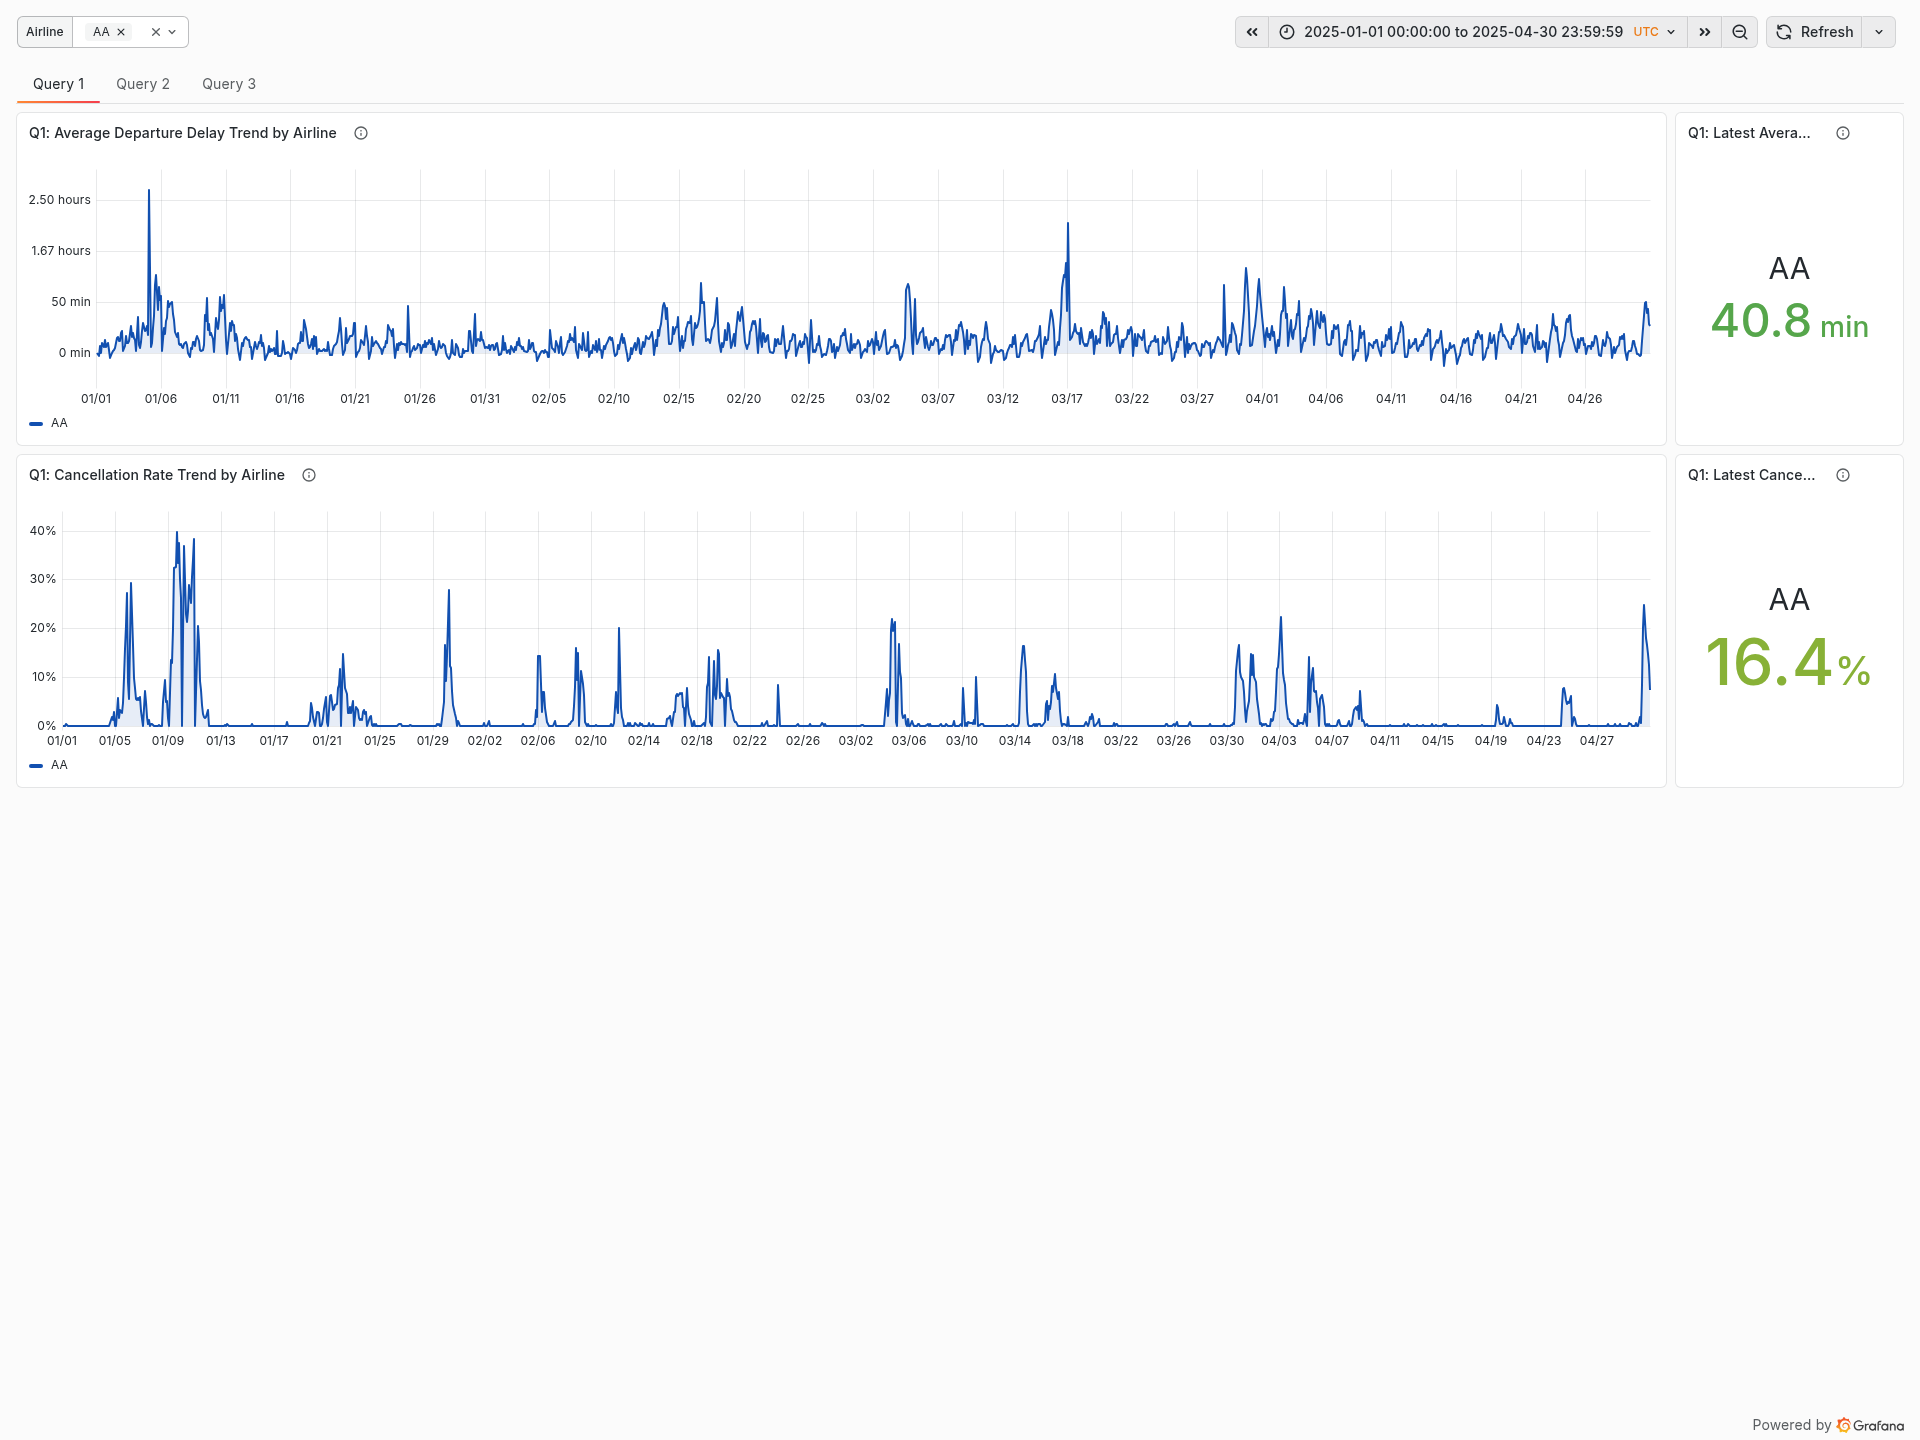
\includegraphics[width=\linewidth,height=0.45\textheight,keepaspectratio]{../Results/plots/Q1_AA_l0.png}
            \vskip -0.1cm
            {\tiny Q1: Ritardo medio e tasso cancellazioni - American Airlines}
            
            \vspace{0.15cm}
            
            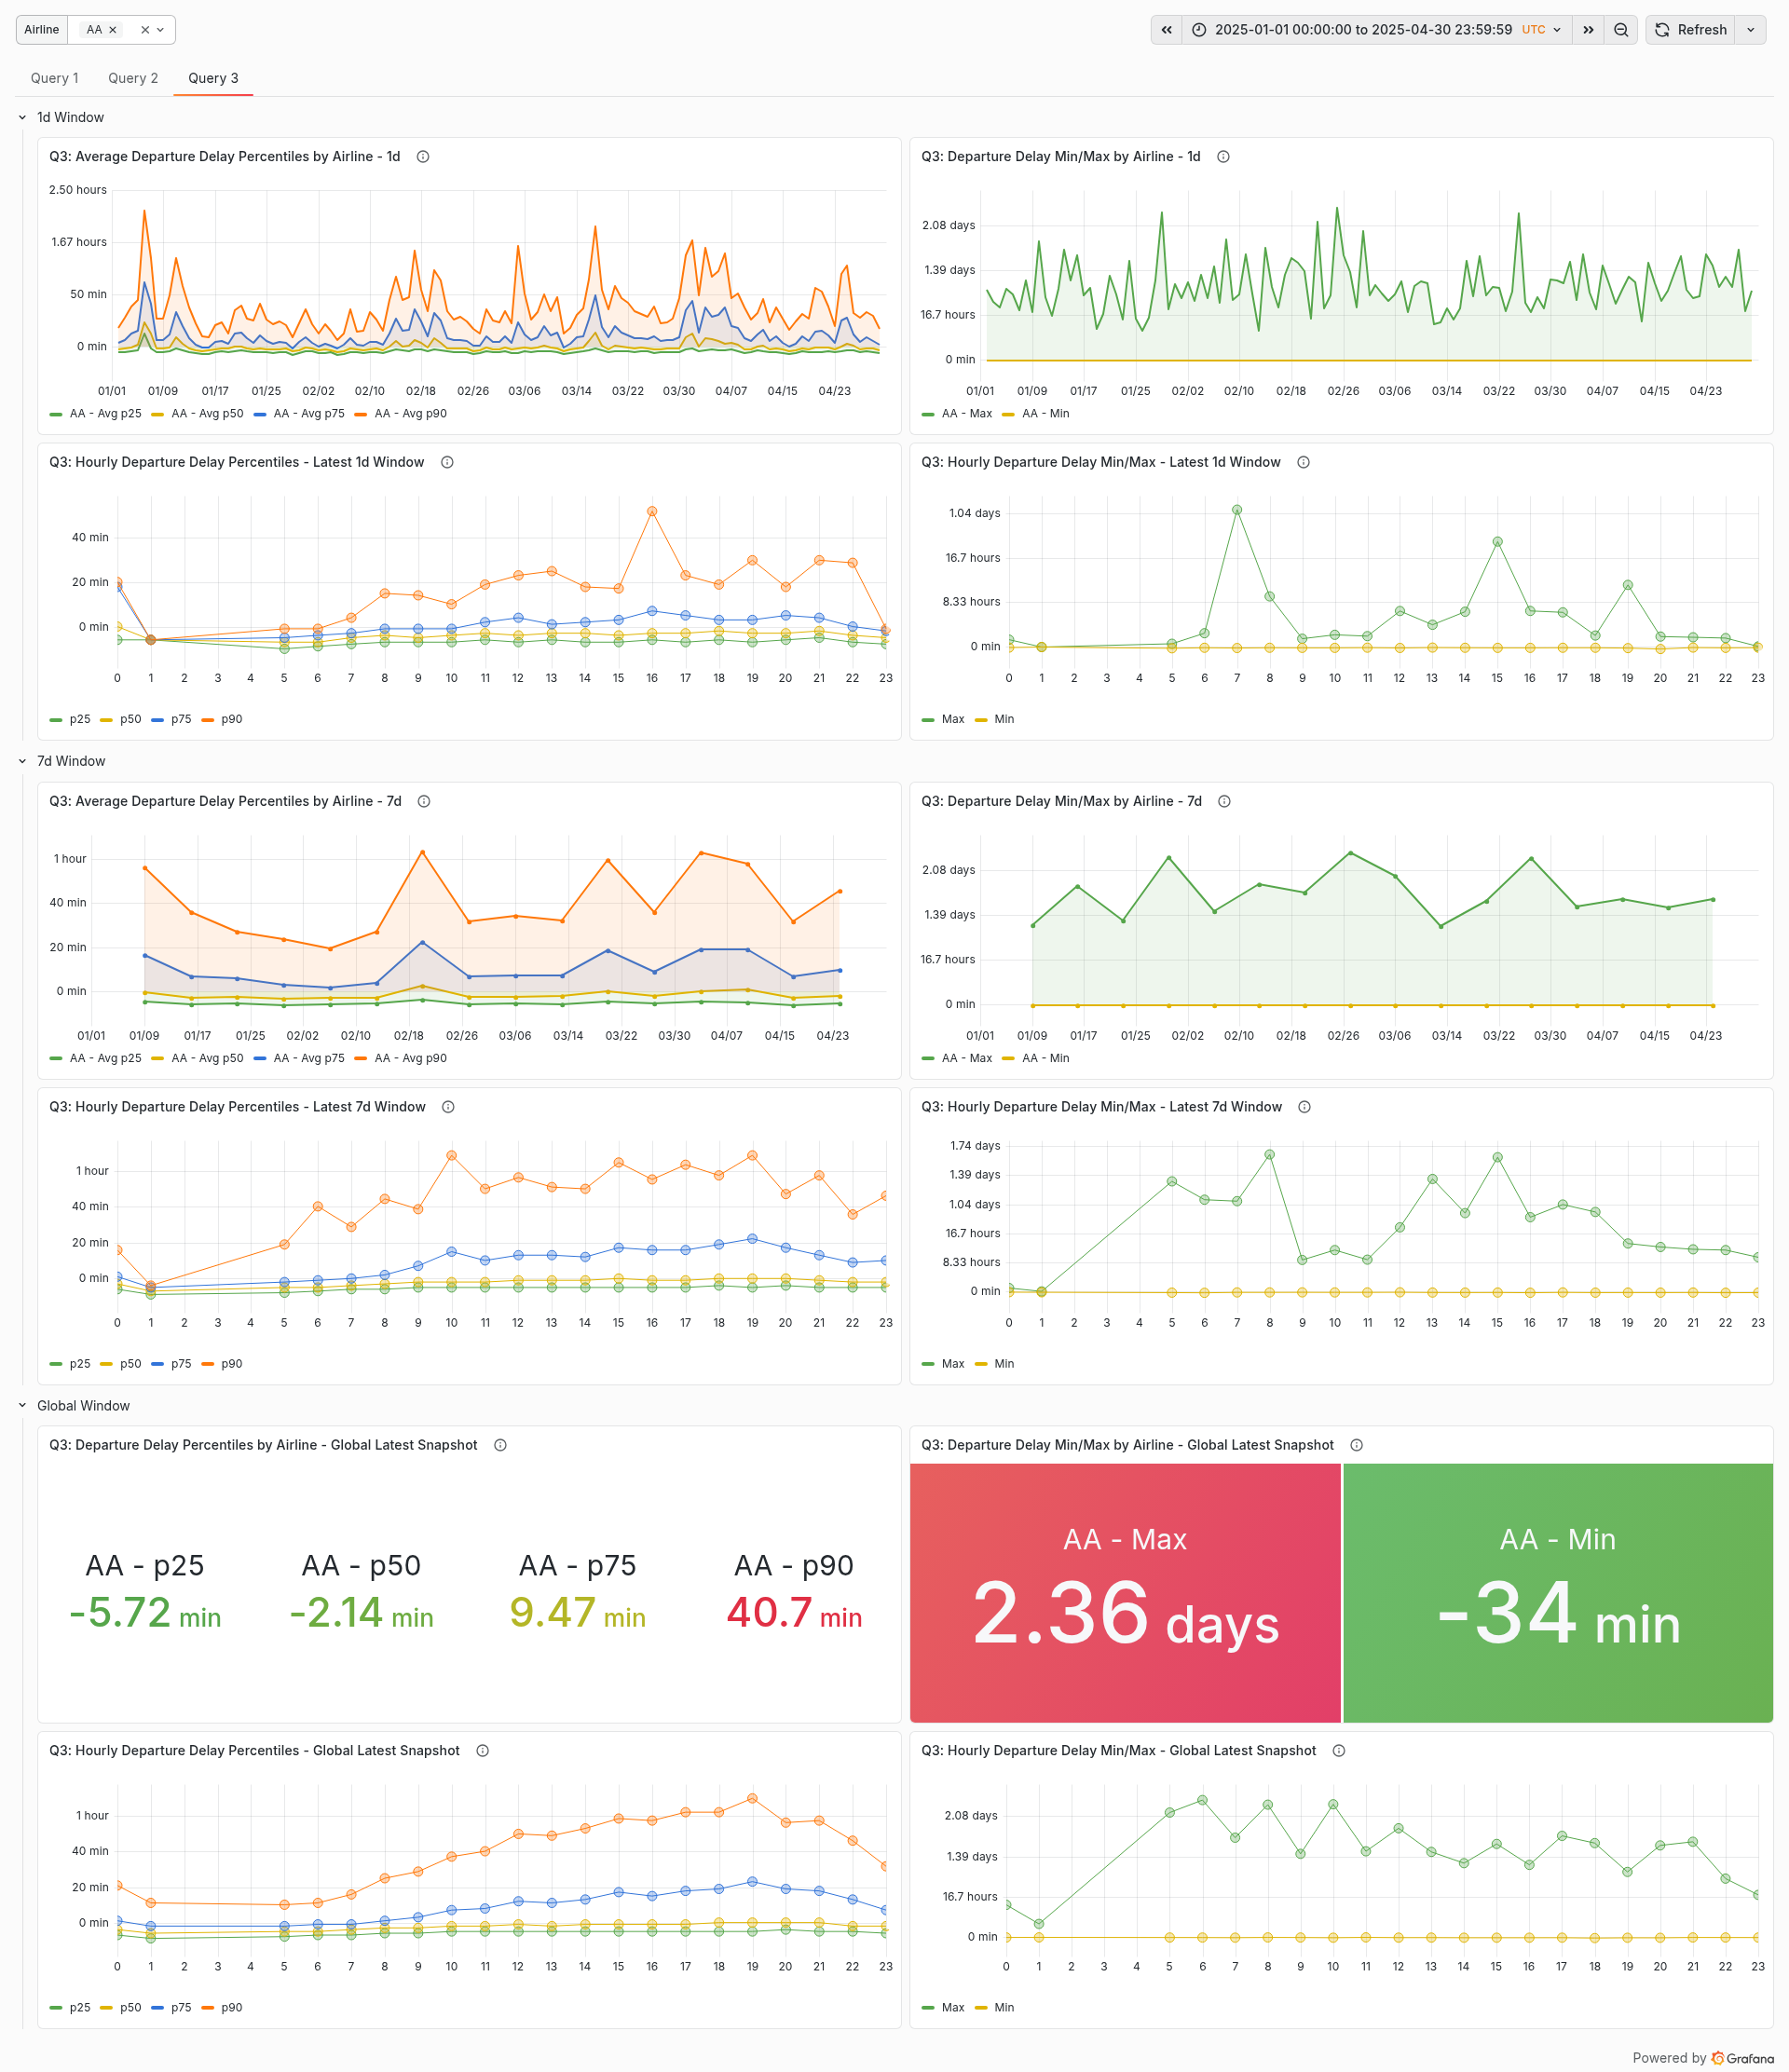
\includegraphics[width=\linewidth,height=0.45\textheight,keepaspectratio]{../Results/plots/Q3_AA_l0.png}
            \vskip -0.1cm
            {\tiny Q3: Percentili su finestra giornaliera - American Airlines}
        \end{column}

        \begin{column}{0.50\textwidth}
            \textbf{Dinamiche Temporali e Ritardi}
            \begin{itemize}
                \footnotesize
                \item \textbf{Query 1 (Performance)}: Presenza di forti picchi intermittenti e localizzati di ritardo e cancellazioni (associabili ad eventi meteo o operativi specifici). Profili nettamente diversi tra i vettori.
                \item \textbf{Query 3 (Percentili con DDSketch)}:
                \begin{itemize}
                    \scriptsize
                    \item Distribuzione fortemente asimmetrica a destra. La mediana è prossima allo zero (la maggior parte dei voli è in orario), ma il 90-esimo percentile sale a decine di minuti con picchi massimi ad ore.
                    \item \textbf{Propagazione dei ritardi}: L'analisi oraria mostra un progressivo peggioramento delle code di ritardo nelle fasce pomeridiane e serali, a causa del ritardo accumulato dagli aeromobili sulle rotte precedenti della giornata.
                \end{itemize}
            \end{itemize}
        \end{column}
    \end{columns}
\end{frame}

\begin{frame}{Risultati Analitici: Query 2 e Granularità}
    \begin{columns}[c]
        \begin{column}{0.48\textwidth}
            \centering
            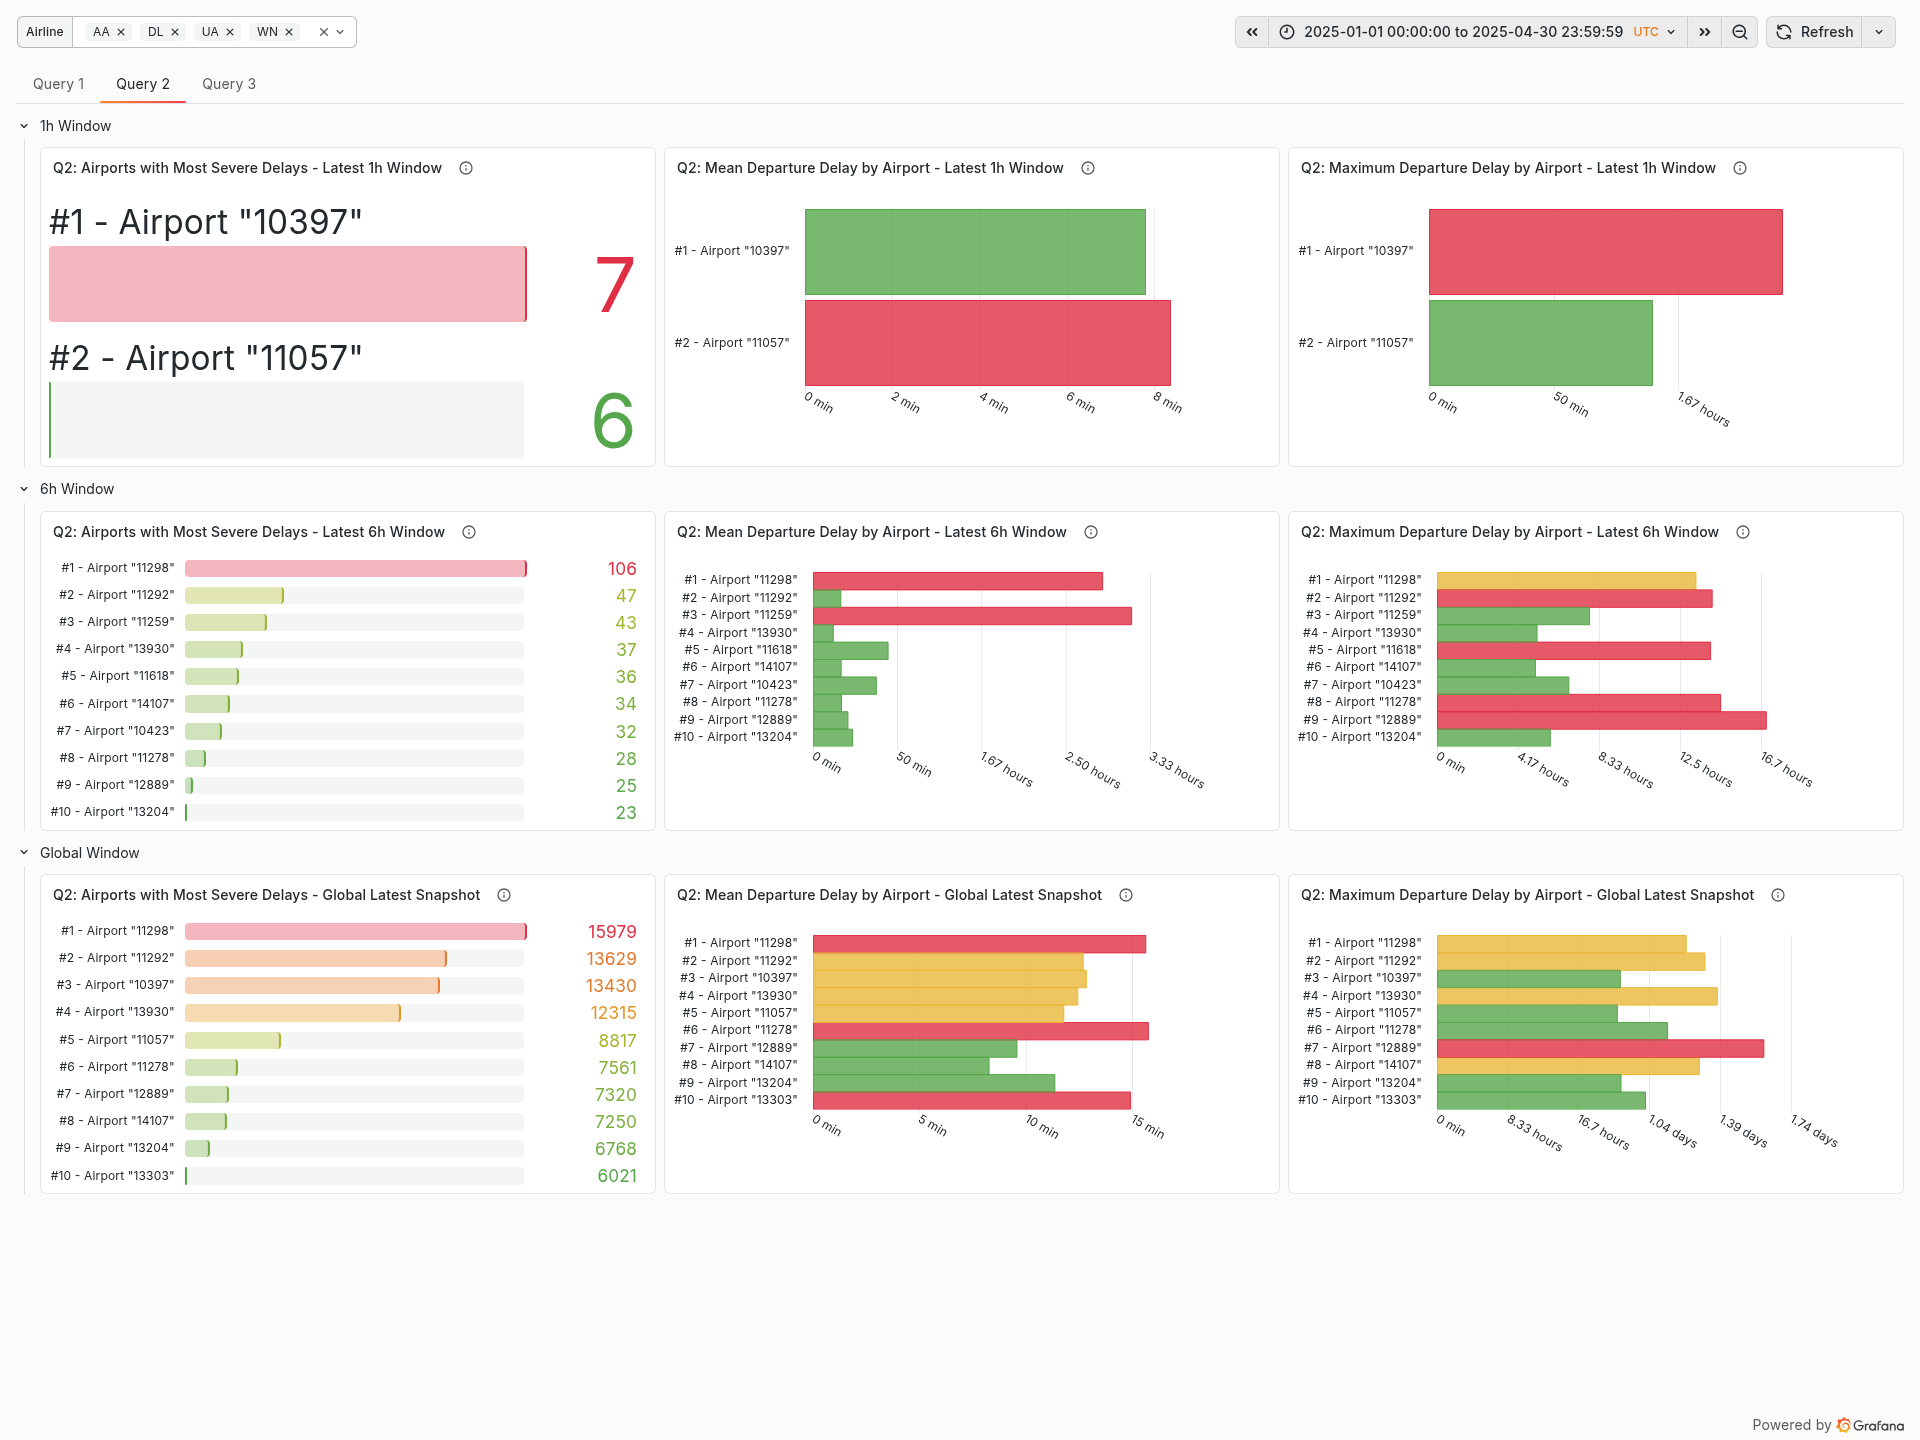
\includegraphics[width=\linewidth,height=0.33\textheight,keepaspectratio]{../Results/plots/Q2_l0.png}
            \vskip -0.1cm
            {\tiny Q2: Classifica aeroporti - Finestra 1 Ora}
            
            \vspace{0.15cm}
            
            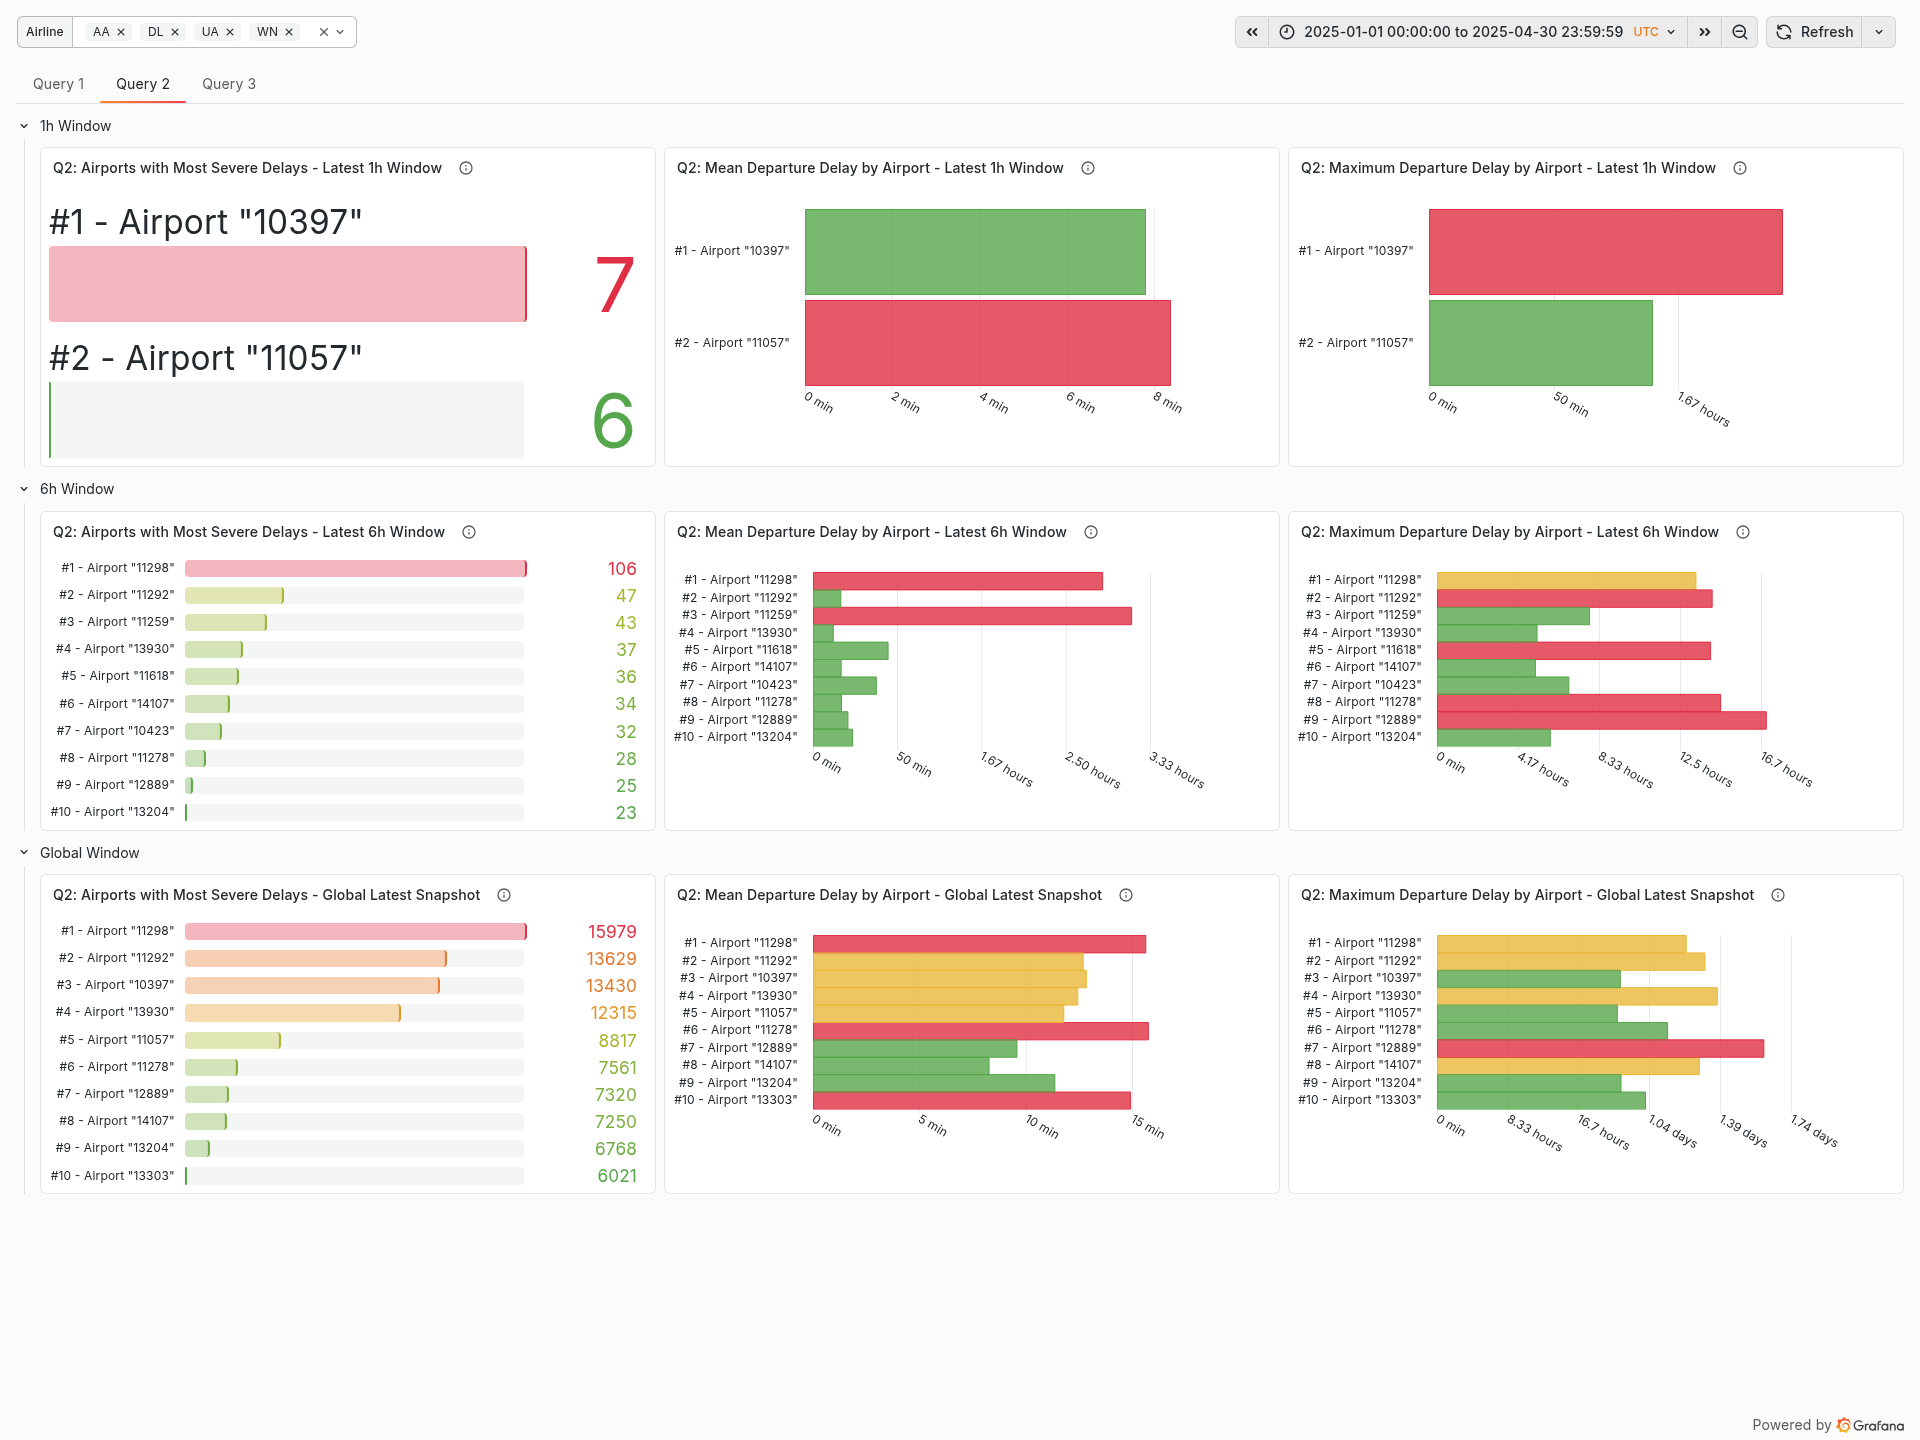
\includegraphics[width=\linewidth,height=0.33\textheight,keepaspectratio]{../Results/plots/Q2_l0.png}
            \vskip -0.1cm
            {\tiny Q2: Classifica aeroporti - Finestra Globale}
        \end{column}

        \begin{column}{0.50\textwidth}
            \textbf{Volatilità vs Stabilità delle Finestre}
            \begin{itemize}
                \footnotesize
                \item \textbf{Finestra a 1 Ora}:
                \begin{itemize}
                    \scriptsize
                    \item Estremamente volatile. Poche decine di voli per finestra consentono a solo due aeroporti di superare la soglia minima di ritardo.
                    \item Adatta per reattività immediata o allarmi operativi in tempo reale.
                \end{itemize}
                \item \textbf{Finestra Globale}:
                \begin{itemize}
                    \scriptsize
                    \item Estremamente stabile e rappresentativa dei trend infrastrutturali di lungo periodo.
                    \item Dominata dagli hub strategici degli Stati Uniti: l'aeroporto \texttt{11298} (Dallas-Fort Worth) totalizza oltre $15.900$ ritardi gravi, seguito da \texttt{11292} (Denver) con $\approx 13.600$ e \texttt{10397} (Atlanta) con $\approx 13.400$.
                \end{itemize}
            \end{itemize}
        \end{column}
    \end{columns}
\end{frame}

\begin{frame}{Impatto della Perdita Dati}
    \begin{columns}[c]
        \begin{column}{0.48\textwidth}
            \centering
            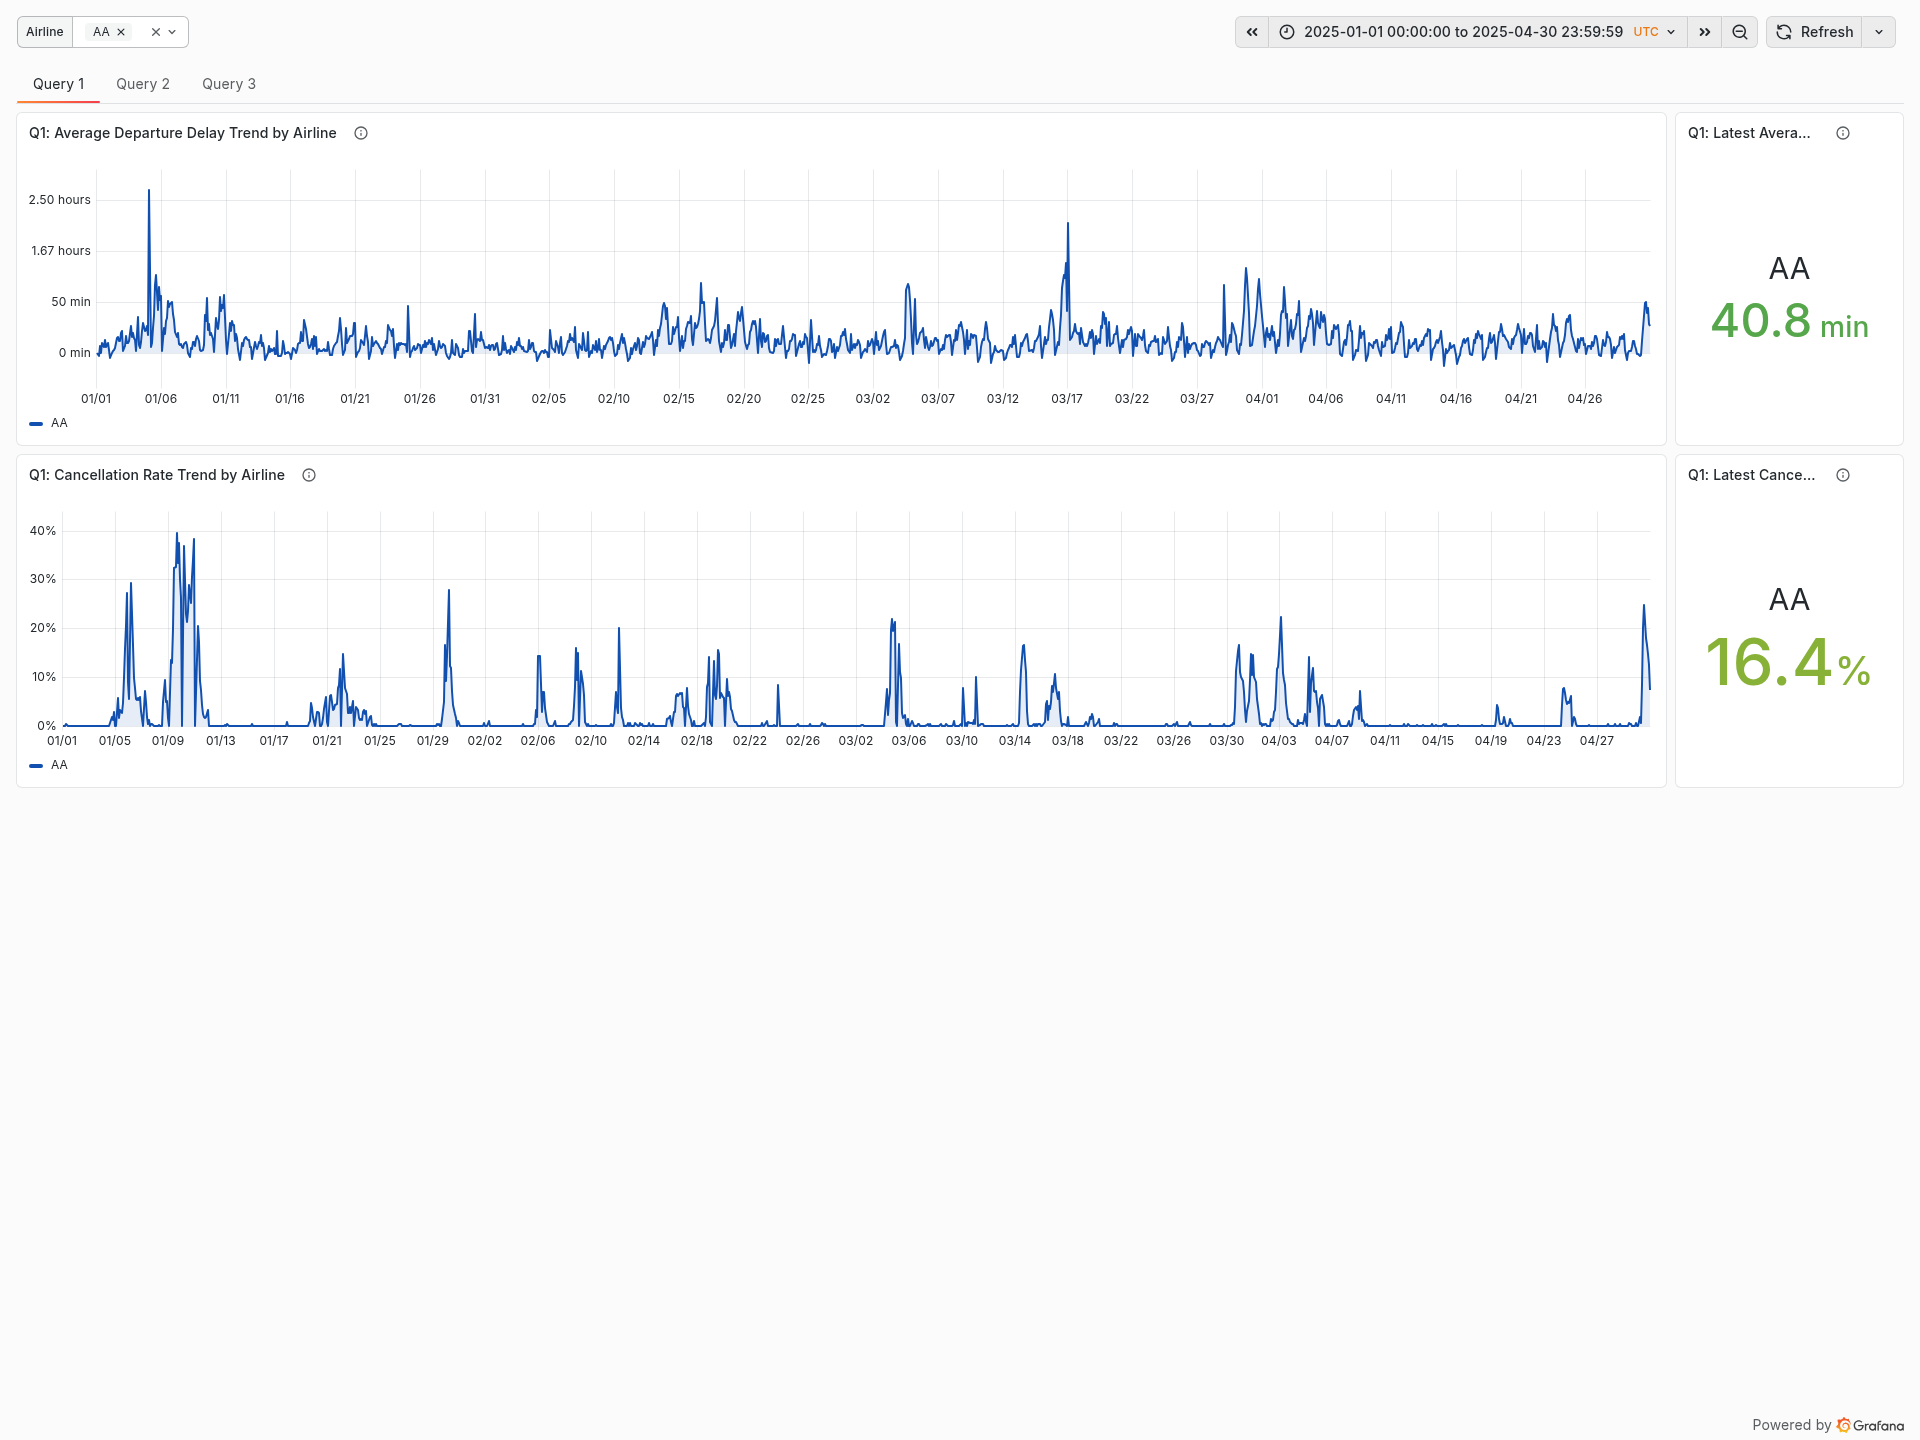
\includegraphics[width=\linewidth,height=0.45\textheight,keepaspectratio]{../Results/plots/Q1_AA_l10.png}
            \vskip -0.1cm
            {\tiny Q1 con perdita del 10\% - American Airlines}
            
            \vspace{0.15cm}
            
            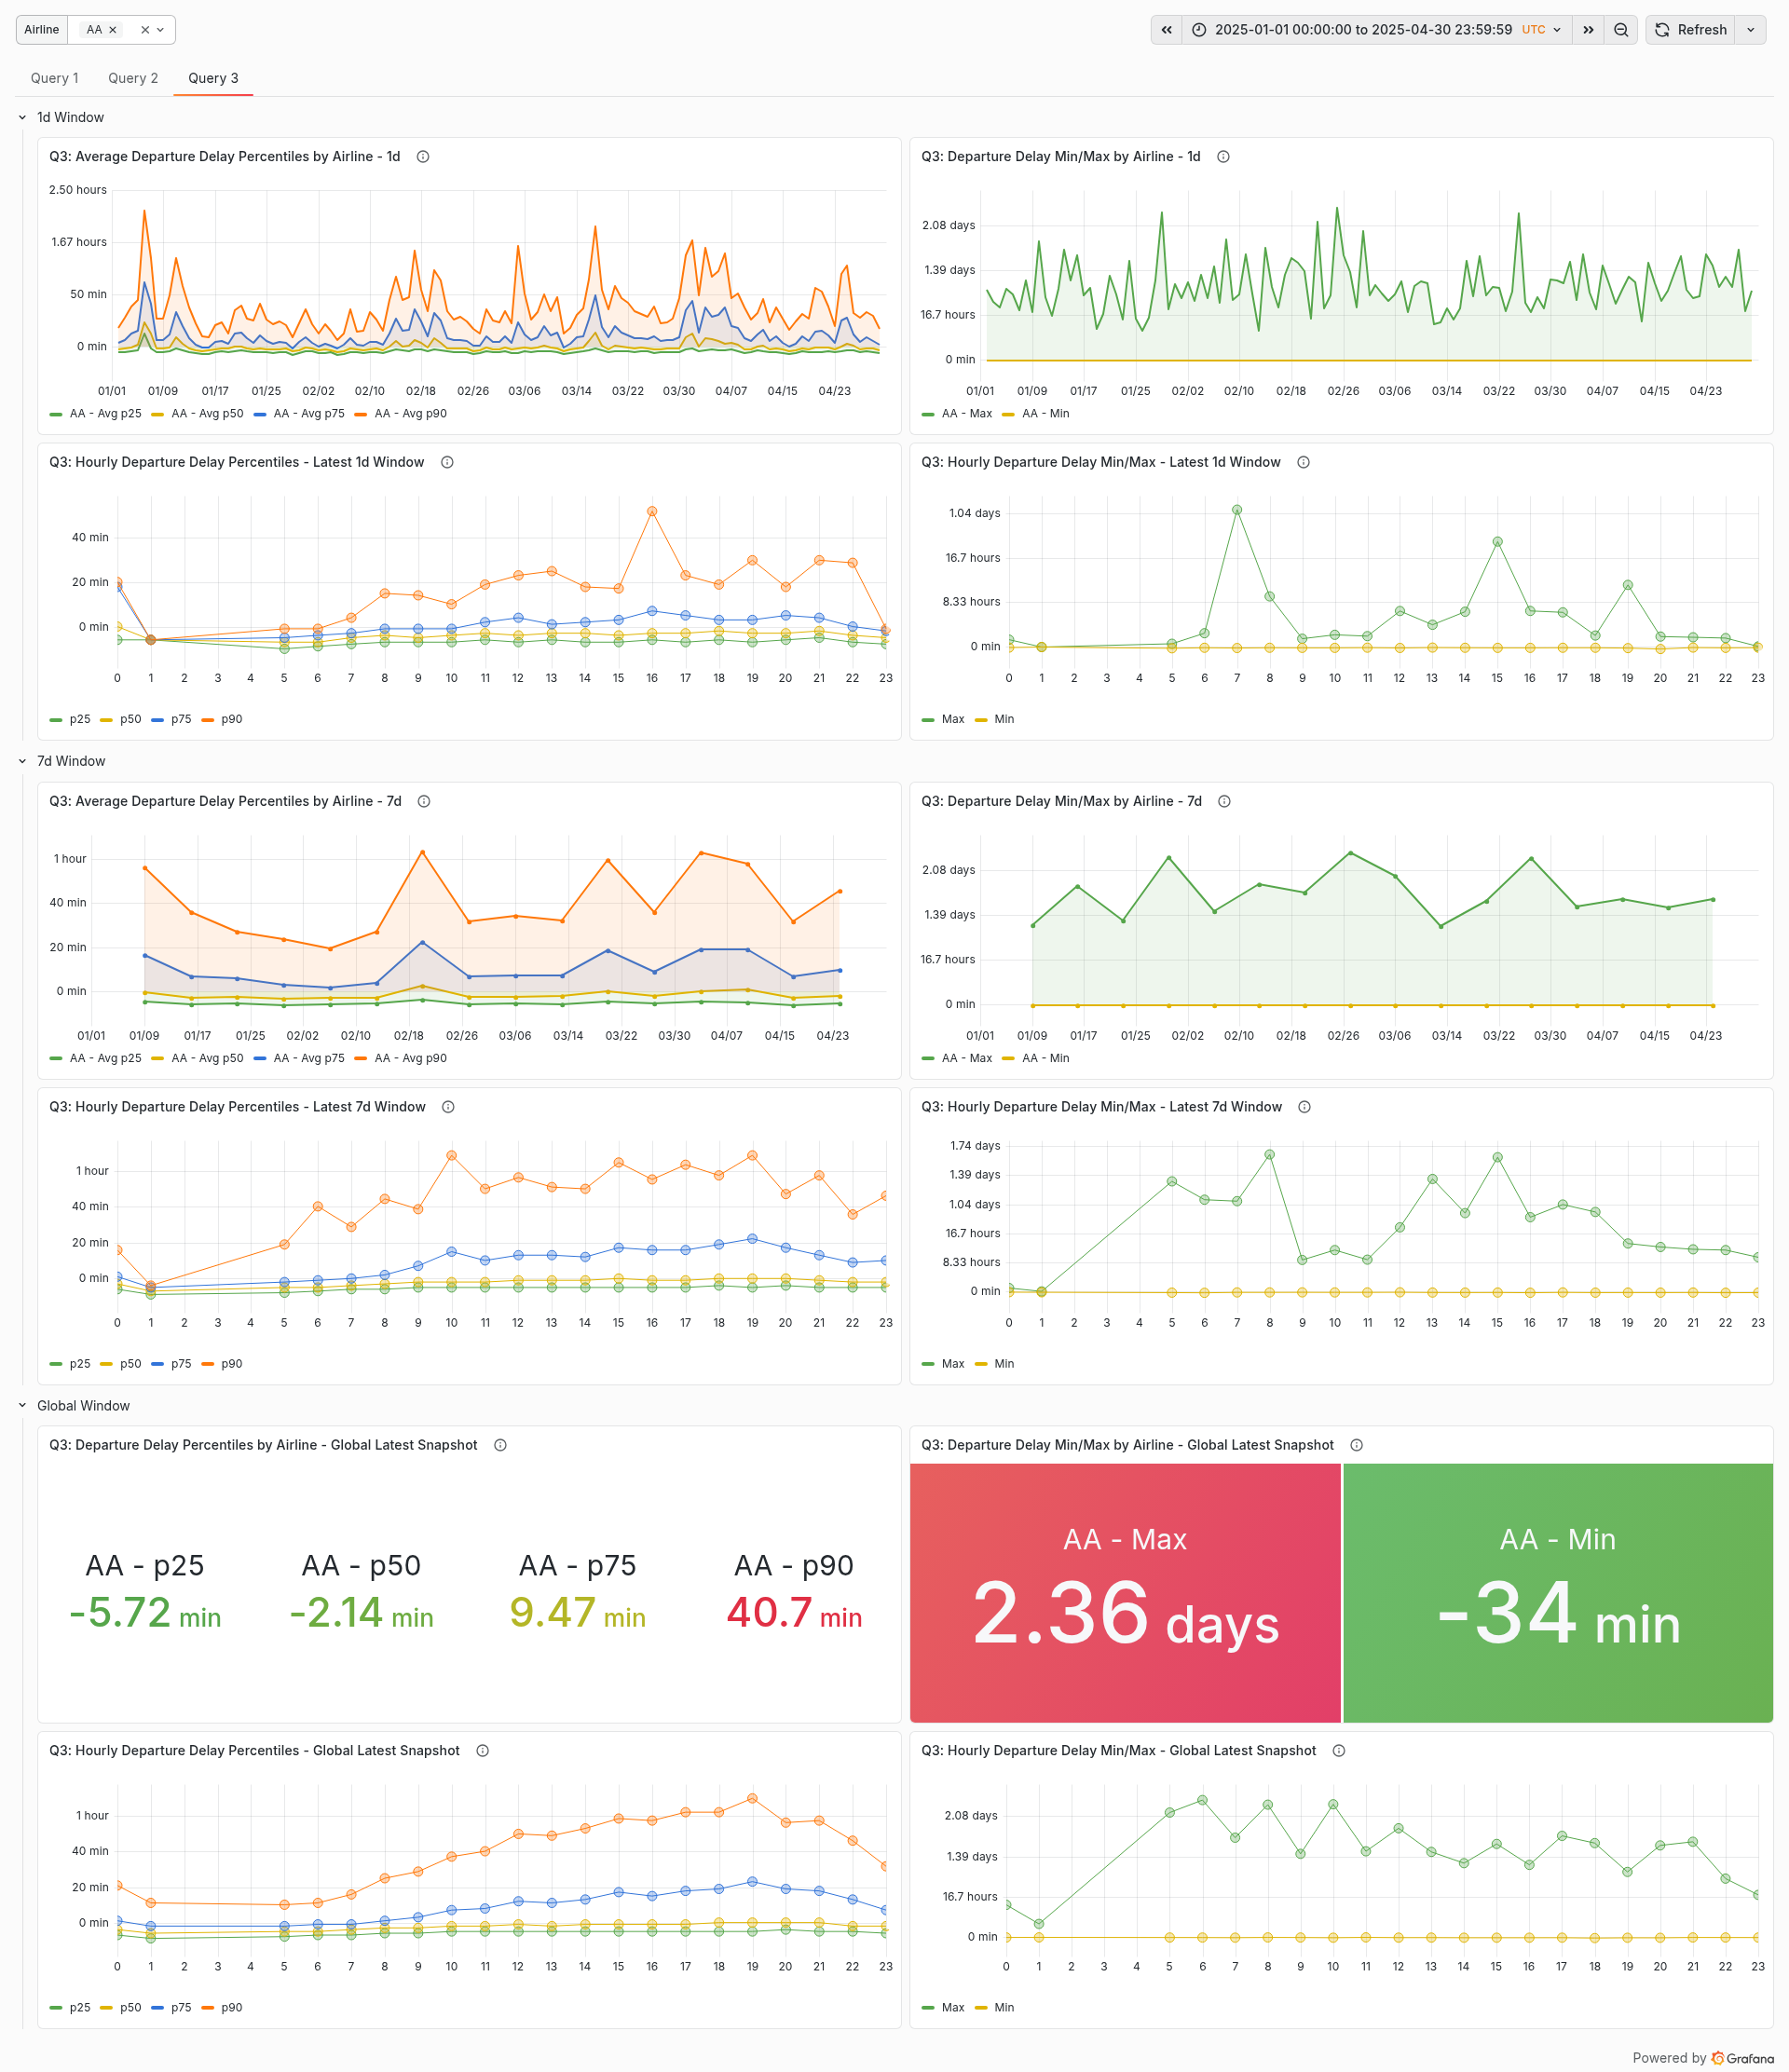
\includegraphics[width=\linewidth,height=0.45\textheight,keepaspectratio]{../Results/plots/Q3_AA_l10.png}
            \vskip -0.1cm
            {\tiny Q3 con perdita del 10\% - American Airlines}
        \end{column}

        \begin{column}{0.50\textwidth}
            \textbf{Confronto Completo vs Lossy}
            \begin{itemize}
                \footnotesize
                \item \textbf{Campagna sperimentale}: Iniezione di una perdita casuale ed uniforme del 10\% sui messaggi all'ingresso di Kafka.
                \item \textbf{Osservazioni}:
                \begin{itemize}
                    \scriptsize
                    \item I profili temporali, i trend generali dei ritardi orari e le stime geometriche dei percentili non mostrano scostamenti sistematici rilevanti.
                    \item Le classifiche degli aeroporti mantengono inalterate le prime posizioni, con variazioni minime nei conteggi assoluti.
                \end{itemize}
                \item \textbf{Valutazione statistica}: La perdita casuale uniforme riduce solo la numerosità del campione ma non introduce distorsioni sistematiche (*bias*).
                \item \textbf{Alert}: Una perdita correlata (es. mirata solo a certe fasce orarie o compagnie) avrebbe invece compromesso radicalmente l'affidabilità analitica.
            \end{itemize}
        \end{column}
    \end{columns}
\end{frame}

% --- CONCLUSIONI ---
\begin{frame}{Conclusioni e Sviluppi Futuri}
    \textbf{Conclusioni}
    \begin{itemize}
        \item \textbf{Ecosistema Streaming Scalabile}: La pipeline in tempo reale sostiene carichi elevati (oltre 8.000 eventi/s) in event-time garantendo consistenza logica e latenze stabili.
        \item \textbf{Infrastruttura di Stato efficiente}: Il bilanciamento tra local-global aggregation e l'uso di DDSketch limita l'impronta di memoria e massimizza l'efficienza degli shuffle di rete.
        \item \textbf{Resilienza e Consistenza}: L'exactly-once interno di Flink combinato con l'idempotenza di InfluxDB fornisce garanzie end-to-end senza pagare l'overhead delle transazioni distribuite su Kafka.
    \end{itemize}

    \vspace{0.3cm}

    \textbf{Sviluppi Futuri}
    \begin{itemize}
        \item \textbf{Watermark Adattivi}: Sviluppo di politiche dinamiche di watermarking che si adattino alla latenza di rete rilevata real-time.
        \item \textbf{Stress Testing}: Campagne di test volte a saturare fisicamente Flink per misurare il comportamento in presenza di *backpressure*.
        \item \textbf{Transactional Kafka}: Integrazione del protocollo a due fasi (2PC) per transazioni atomiche native a livello di sink.
    \end{itemize}
\end{frame}

\begin{frame}
    \vfill
    \begin{center}
        \huge \textbf{Grazie per l'attenzione} \\
        \vspace{1.5cm}
        
\includegraphics[width=0.35\textwidth]{logos/logo_tor_vergata}
    \end{center}
    \vfill
\end{frame}

\end{document}
